\chapter{Introduction}
\label{chapter:introduction}

\section{Problem description}

The use of IoT devices is growing rapidly due to their low price, connectivity capabilities, and variety of sensors and applications. \\
A large number of brands and manufacturers use electronics and software from OEM suppliers  which are, sometimes, vulnerable to known attacks and exploits. These known vulnerabilities makes that kind of devices perfect candidates for being infected, controlled and added as part of botnets, commonly used to perform DDoS attacks \cite{perakovic2015analysis}.

Online hacker forums have been, since their inception, meeting places in which to share information. When it comes to DDOS attacks, they can be a valuable source of information on how to protect. But, as stated by Yue et al. \cite{yue2019see}, they have often also been a source of information on how to carry out attacks.

Given the great potential for harm of these botnets and the increasing number of DDoS attacks that currently occurs, it is important to understand how this information is shared, and the economics behind it. That knowledge could be valuable in order to build \textit{prevent \& protect} strategies.

\section{Objectives}

Current work main purpose is know how the sale of accecss to IoT devices for DDoS has evolved over time.
To do so, the key points to be analyzed are:

\begin{itemize}
\item Identifying main underground forum sites on which IoT access are being sold.
\item Know the importance of these services vs other type of criminal offered services.
\item Measure how much underground communities are interested in these services in terms of supply vs demand.
\item Getting details about how these services are monetized.
\end{itemize}

\section{State of the art}

There are works focused on measuring how \textit{Cybercrime-as-a-Service} (CaaS) are sold in underground forums \cite{measuringCaaS}. These works are a valuable source in order to understand how CaaS are sold in underground forums, but doesn't focus on sale of IoT devices access for DDoS. \\
Also there are some studies regarding \textit{Cybercrime-as-a-Service} (CaaS) focused on Sale of access IoT devices for DDoS, main topic of this work. But these works are focused in other channels like Telegram and Discord \cite{booters}, not just for underground forums.

Some private security companies, have analysed underground communities around the world in order to get a view on how IoT devices are being used for criminal purposes. Hilt et al. in their analysis about "IoT in the Cybercrime Underground" \cite{trendMicroConclusions} (Trend Micro research), stated that \textquote{nation-states and more dangerous threat actors are also
infecting IoT devices to use them as DoS platforms}. In that article they shows some good examples as the sale of an IoT botnet in Hack Forums \cite{trendMicroHackForums}.

\begin{figure}
	\centering
	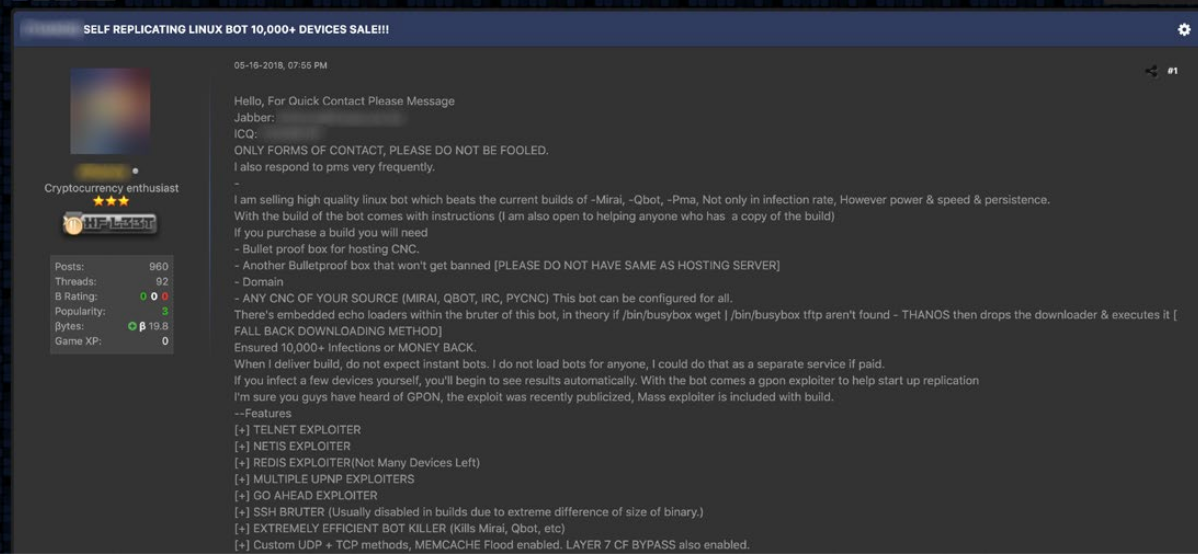
\includegraphics[width=0.8\textwidth]{figs/hf_sale_iot.png}
	\caption{IoT botnet for sale on Hack Forums}
	\label{fig:hf_sale_iot}
\end{figure}

\subsection{Forums}
\label{sec:forums}

First it is needed to identify most relevant underground forums. As stated by work done by Akyazi, U., van Eeten, M. J. G., \& Hernandez Ganan, C \cite{measuringCaaS}, based on \textit{CrimeBB} \cite{crimeBB} database from Cambridge Cybercrime Centre, most relevant underground forums (in order of relevance) are:

\vspace{0.5cm}

\begin{tabular}{llrrrr}
    \hline
    Forum & Language & Members & Threads & Posts & Oldest \\
    \hline
    Hackforums & EN & 573925 & 3856143 & 40196641 & 01/2007 \\
    Multiplayer Game Hacking & EN & 452186 & 739527 & 8907938 & 12/2005 \\
    Antichat & RU & 77865 & 242408 & 2449221 & 05/2002 \\
    RaidForums & EN & 43278 & 33100 & 124776 & 03/2015 \\
    Offensive Community & EN & 10593 & 18436 & 58779 & 06/2012 \\
    SafeSkyHacks & EN & 7378 & 12892 & 26842 & 03/2013 \\
    Kernelmode & EN & 1441 & 3144 & 25024 & 03/2010 \\
    Garage4Hackers & EN & 872 & 2096 & 7697 & 07/2010 \\
    Stresserforums & EN & 764 & 708 & 7069 & 04/2017 \\
    Greysee & EN & 440 & 1239 & 6969 & 06/2015 \\
    \hline
\end{tabular}
\\
\\
The information collected in crimeBB, with the activity of the underground forums, is a vast data set with millions of records. Given the impossibility of covering all that information in this work, it is decided to analyze the information contained in Hack Forums, as it is the largest.
